\iffalse
  \title{Assignment1 EE24BTECH11025}
  \author{GEEDI HARSHA VARDHAN}
  \section{ph}
  \chapter{2014}
\fi

\item
A student is required to demonstrate a high level of comprehension of the subject, especially in the social sciences.The word closest in meaning to comprehension is

\begin{enumerate}
\item  understanding
\item  meaning
\item  concentration
\item  stability
\end{enumerate}

\item 
Choose the most appropriate word from the options given below to complete the following sentence.

One of his biggest was his ability to forgive.

\begin{enumerate}
\item  vice
\item  virtues
\item  choices
\item  strength
\end{enumerate}

\item 
Rajan was not happy that Sajan decided to do the project on his own. On observing his unhappiness, Sajan explained to Rajan that he preferred to work independently.

Which one of the statements below is logically valid and can be inferred from the above sentences?

\begin{enumerate}
\item  Rajan has decided to work only in a group.
\item  Rajan and Sajan were formed into a group against their wishes.
\item  Sajan had decided to give in to Rajan's request to work with him.
\item  Rajan had believed that Sajan and he would be working together.
\end{enumerate}

\item  If $y = 5x^2+ 3$, then the tangent at $x = 0$, $y = 3$

\begin{enumerate}
\item  passes through $x = 0$, $y = 0$
\item  has a slope of +1
\item  is parallel to the x-axis
\item  has a slope of -1
\end{enumerate}

\item 
A foundry has a fixed daily cost of Rs 50,000 whenever it operates and a variable cost of Rs 800Q, where $Q$ is the daily production in tonnes. What is the cost of production in Rs per tonne for a daily production of 100 tonnes?

\item Find the odd one in the following group: ALRVX, EPVZB, ITZDF, OYEIK

\begin{enumerate}
    \item ALRVX
    \item EPVZB
    \item ITZDF
    \item OYEIK
\end{enumerate}


\item Anuj, Bhola, Chandan, Dilip, Eswar, and Faisal live on different floors in a six-storeyed building (the ground floor is numbered 1, the floor above it 2, and so on). Anuj lives on an even-numbered floor. Bhola does not live on an odd-numbered floor. Chandan does not live on any of the floors below Faisal's floor. Dilip does not live on floor number 2. Eswar does not live on a floor immediately above or immediately below Bhola. Faisal lives three floors above Dilip. Which of the following floor-person combinations is correct?


\begin{table}
\centering
\begin{tabular}[12pt]{|c|c|c|c|c|c|c|c|}
\hline
Option & Anuj & Bhola & Chandan & Dilip & Eswar & Faisal \\
\hline
(A) & 6 & 2 & 5 & 1 & 3 & 4 \\
\hline
(B) & 2 & 6 & 5 & 1 & 3 & 4 \\
\hline
(C) & 4 & 2 & 6 & 3 & 1 & 5 \\
\hline
(D) & 2 & 4 & 6 & 1 & 3 & 5 \\
\hline
\end{tabular}
\end{table}





\item The smallest angle of a triangle is equal to two thirds of the smallest angle of a quadrilateral. The ratio between the angles of the quadrilateral is 3:4:5:6. The largest angle of the triangle is twice its smallest angle. What is the sum, in degrees, of the second largest angle of the triangle and the largest angle of the quadrilateral?

\item One percent of the people of country $X$ are taller than 6 ft. Two percent of the people of country $Y$ are taller than 6 ft. There are thrice as many people in country $X$ as in country $Y$. Taking both countries together, what is the percentage of people taller than 6 ft?
\begin{enumerate}

    \item 3.0
    \item 2.5
    \item 1.5
    \item 1.25
\end{enumerate}

\item The monthly rainfall chart based on 50 years of rainfall in Agra is shown in the following figure. Which of the following are true? ($k$ percentile is the value such that $k$ percent of the data fall below that value)

\begin{figure}[H]
\centering
\pgfplotsset{compat=1.17}


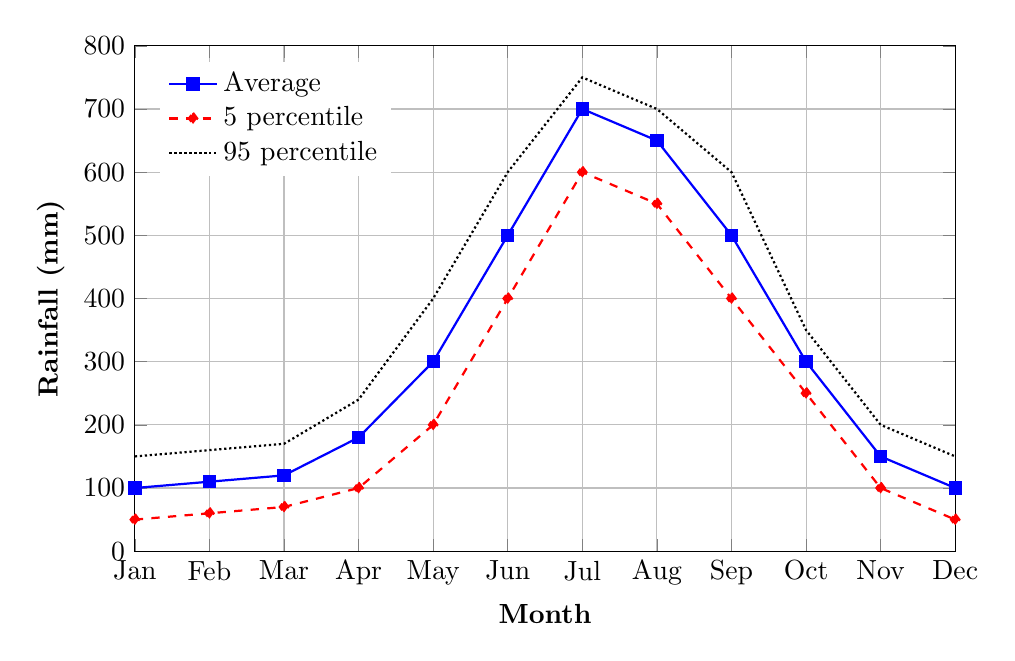
\begin{tikzpicture}
\begin{axis}[
    width=12cm, height=8cm,
    xlabel={\textbf{Month}},
    ylabel={\textbf{Rainfall (mm)}},
    xmin=1, xmax=12,
    ymin=0, ymax=800,
    xtick={1,2,3,4,5,6,7,8,9,10,11,12},
    xticklabels={Jan, Feb, Mar, Apr, May, Jun, Jul, Aug, Sep, Oct, Nov, Dec},
    ytick={0, 100, 200, 300, 400, 500, 600, 700, 800},
    legend pos=north west,
    legend cell align={left},
    legend style={draw=none},
    grid=both
]

% Average Line
\addplot[
    color=blue,
    mark=square*,
    thick
]
coordinates {
    (1,100) (2,110) (3,120) (4,180) (5,300) (6,500) 
    (7,700) (8,650) (9,500) (10,300) (11,150) (12,100)
};
\addlegendentry{Average}

% 5 Percentile Line
\addplot[
    color=red,
    dashed,
    mark=diamond*,
    thick
]
coordinates {
    (1,50) (2,60) (3,70) (4,100) (5,200) (6,400) 
    (7,600) (8,550) (9,400) (10,250) (11,100) (12,50)
};
\addlegendentry{5 percentile}

% 95 Percentile Line
\addplot[
    color=black,
    densely dotted,
    thick
]
coordinates {
    (1,150) (2,160) (3,170) (4,240) (5,400) (6,600) 
    (7,750) (8,700) (9,600) (10,350) (11,200) (12,150)
};
\addlegendentry{95 percentile}

\end{axis}
\end{tikzpicture}

\end{figure}


\begin{enumerate}
    \item On average, it rains more in July than in December.
    \item Every year, the amount of rainfall in August is more than that in January.
    \item July rainfall can be estimated with better confidence than February rainfall.
    \item In August, there is at least 500 mm of rainfall.
\end{enumerate}

\begin{enumerate}
    \item (i) and (ii)
    \item (i) and (iii)
    \item (ii) and (iii)
    \item (iii) and (iv)
\end{enumerate}
 \item The unit vector perpendicular to the surface $x^2 + y^2 + z^2 = 3$ at the point (1,1,1) is
        \begin{enumerate}
            \item $\frac{\hat{x} + \hat{y} - \hat{z}}{\sqrt{3}}$
            \item $\frac{\hat{x} - \hat{y} + \hat{z}}{\sqrt{3}}$
            \item $\frac{\hat{x} - \hat{y} - \hat{z}}{\sqrt{3}}$
            \item $\frac{\hat{x} + \hat{y} + \hat{z}}{\sqrt{3}}$
        \end{enumerate}

    \item Which one of the following quantities is invariant under Lorentz transformation?
        \begin{enumerate}
            \item Charge density
            \item Charge
            \item Current
            \item Electric field
        \end{enumerate}

    \item The number of normal Zeeman splitting components of $P \rightarrow D$ transition is
        \begin{enumerate}
            \item 3
            \item 4
            \item 8
            \item 9
        \end{enumerate}

